% ===========================================================================
%  TikuOS — TikuKits DS: Circular Log for Embedded Systems
%  Beamer Presentation
% ===========================================================================
\documentclass[aspectratio=169, 10pt]{beamer}

% ---- Theme ----------------------------------------------------------------
\usetheme{Madrid}
\usecolortheme{whale}
\setbeamertemplate{navigation symbols}{}
\setbeamertemplate{footline}{%
  \leavevmode\hbox{%
    \begin{beamercolorbox}[wd=.33\paperwidth,ht=2.5ex,dp=1ex,center]{author in head/foot}%
      \usebeamerfont{author in head/foot}\insertshortauthor
    \end{beamercolorbox}%
    \begin{beamercolorbox}[wd=.34\paperwidth,ht=2.5ex,dp=1ex,center]{title in head/foot}%
      \usebeamerfont{title in head/foot}\insertshorttitle
    \end{beamercolorbox}%
    \begin{beamercolorbox}[wd=.33\paperwidth,ht=2.5ex,dp=1ex,right]{date in head/foot}%
      \usebeamerfont{date in head/foot}\insertshortdate{}\hspace*{2em}%
      \insertframenumber{}/\inserttotalframenumber\hspace*{2ex}
    \end{beamercolorbox}}%
  \vskip0pt%
}

% ---- Packages -------------------------------------------------------------
\usepackage{listings}
\usepackage{graphicx}
\usepackage{hyperref}
\usepackage{booktabs}
\usepackage{multirow}
\usepackage{tikz}
\usetikzlibrary{arrows.meta, positioning, shapes.geometric, calc,
                decorations.pathreplacing, fit}
\usepackage{amsmath}

% ---- Code listing style ---------------------------------------------------
\lstset{
  basicstyle=\ttfamily\scriptsize,
  keywordstyle=\color{blue}\bfseries,
  commentstyle=\color{gray},
  stringstyle=\color{red!70!black},
  showstringspaces=false,
  breaklines=true,
  frame=single,
  rulecolor=\color{black!30},
  backgroundcolor=\color{blue!3},
  tabsize=4,
}
\lstdefinestyle{cstyle}{
  language=C,
  morekeywords={uint8_t,uint16_t,uint32_t,int32_t,int16_t,
                tiku_kits_ds_elem_t,
                TIKU_KITS_DS_OK,TIKU_KITS_DS_ERR_NULL,
                TIKU_KITS_DS_ERR_PARAM,TIKU_KITS_DS_ERR_BOUNDS,
                TIKU_KITS_DS_ERR_EMPTY,TIKU_KITS_DS_ERR_FULL,
                TIKU_KITS_DS_ERR_NOTFOUND,
                TIKU_KITS_DS_CIRCLOG_MAX_ENTRIES,
                TIKU_KITS_DS_CIRCLOG_PAYLOAD_SIZE,
                TIKU_KITS_DS_CIRCLOG_LEVEL_DEBUG,
                TIKU_KITS_DS_CIRCLOG_LEVEL_INFO,
                TIKU_KITS_DS_CIRCLOG_LEVEL_WARN,
                TIKU_KITS_DS_CIRCLOG_LEVEL_ERROR,
                TIKU_KITS_DS_CIRCLOG_LEVEL_FATAL,
                NULL,size_t},
}

% ---- Metadata -------------------------------------------------------------
\title[TikuKits DS]{TikuKits DS: Circular Log for Embedded Systems}
\subtitle{Simple. Ubiquitous. Intelligence, Everywhere.}
\author[Ambuj Varshney]{Ambuj Varshney \\ \texttt{ambuj@tiku-os.org}}
\date{\today}

% ===========================================================================
\begin{document}

% ---------------------------------------------------------------------------
\begin{frame}
\titlepage
\end{frame}

% ---------------------------------------------------------------------------
\begin{frame}{Outline}
\tableofcontents
\end{frame}

% ===========================================================================
\section{Motivation}
% ===========================================================================

\begin{frame}{Why Structured Logging on MCUs?}
\begin{columns}[T]
\begin{column}{0.48\textwidth}
\begin{block}{Embedded Use Cases}
\begin{itemize}
  \item \textbf{Post-mortem debugging} --- inspect crash history after reset
  \item \textbf{Event tracing} --- record state transitions with timestamps
  \item \textbf{Error tracking} --- count and categorize faults
  \item \textbf{Field diagnostics} --- read log via UART after deployment
  \item \textbf{FRAM persistence} --- survive power loss
\end{itemize}
\end{block}

\begin{block}{Constraints}
\begin{itemize}
  \item RAM/FRAM is scarce (2--8\,KB)
  \item Must never overflow --- bounded memory usage
  \item $O(1)$ append --- cannot block the main loop
  \item Structured entries for programmatic parsing
\end{itemize}
\end{block}
\end{column}

\begin{column}{0.48\textwidth}
\begin{center}
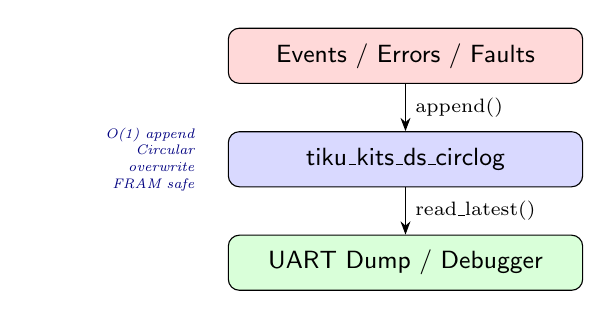
\begin{tikzpicture}[
    >=Stealth, node distance=0.5cm
  ]
  \node[draw, rounded corners, minimum height=0.7cm,
        text centered, font=\small\sffamily, fill=red!15,
        minimum width=4.5cm] (evt) {Events / Errors / Faults};
  \node[draw, rounded corners, minimum height=0.7cm,
        text centered, font=\small\sffamily, fill=blue!15,
        minimum width=4.5cm, below=0.6cm of evt] (cl)
    {tiku\_kits\_ds\_circlog};
  \node[draw, rounded corners, minimum height=0.7cm,
        text centered, font=\small\sffamily, fill=green!15,
        minimum width=4.5cm, below=0.6cm of cl] (dbg)
    {UART Dump / Debugger};
  \draw[->] (evt) -- node[right, font=\scriptsize] {append()} (cl);
  \draw[->] (cl) -- node[right, font=\scriptsize] {read\_latest()} (dbg);

  \node[left=0.3cm of cl, font=\tiny\itshape, text=blue!50!black,
        text width=2cm, align=right] {O(1) append\\Circular\\overwrite\\FRAM safe};
\end{tikzpicture}
\end{center}

\vspace{0.5em}
\begin{alertblock}{Why Not \texttt{printf}?}
\texttt{printf} requires a UART connection, consumes code space
for format strings, and produces no persistent record.
A circular log stores structured entries in FRAM that survive
power loss and can be read at any time.
\end{alertblock}
\end{column}
\end{columns}
\end{frame}

% ===========================================================================
\section{Data Structure}
% ===========================================================================

\begin{frame}[fragile]{The \texttt{tiku\_kits\_ds\_circlog} Structure}
\begin{columns}[T]
\begin{column}{0.48\textwidth}
\begin{lstlisting}[style=cstyle,
  title={ds/circlog/tiku\_kits\_ds\_circlog.h}]
#ifndef TIKU_KITS_DS_CIRCLOG_MAX_ENTRIES
#define TIKU_KITS_DS_CIRCLOG_MAX_ENTRIES 16
#endif

#ifndef TIKU_KITS_DS_CIRCLOG_PAYLOAD_SIZE
#define TIKU_KITS_DS_CIRCLOG_PAYLOAD_SIZE 8
#endif

struct tiku_kits_ds_circlog_entry {
    uint32_t timestamp;
    uint8_t  level;
    uint8_t  tag;
    uint8_t  payload[
        TIKU_KITS_DS_CIRCLOG_PAYLOAD_SIZE];
    uint16_t sequence;
};

struct tiku_kits_ds_circlog {
    struct tiku_kits_ds_circlog_entry
        entries[
        TIKU_KITS_DS_CIRCLOG_MAX_ENTRIES];
    uint16_t head;
    uint16_t count;
    uint16_t capacity;
    uint16_t next_seq;
};
\end{lstlisting}
\end{column}

\begin{column}{0.48\textwidth}
\begin{block}{Entry Fields}
\begin{itemize}
  \item \textbf{timestamp} --- system clock at log time
  \item \textbf{level} --- DEBUG, INFO, WARN, ERROR, FATAL
  \item \textbf{tag} --- module identifier (0--255)
  \item \textbf{payload} --- raw data bytes (configurable size)
  \item \textbf{sequence} --- monotonic counter for ordering
\end{itemize}
\end{block}

\vspace{0.3em}
\begin{block}{Log Levels}
\scriptsize
\begin{tabular}{@{}ll@{}}
\texttt{LEVEL\_DEBUG} (0) & Verbose debug info \\
\texttt{LEVEL\_INFO}  (1) & Normal events \\
\texttt{LEVEL\_WARN}  (2) & Recoverable issues \\
\texttt{LEVEL\_ERROR} (3) & Errors requiring attention \\
\texttt{LEVEL\_FATAL} (4) & Unrecoverable faults \\
\end{tabular}
\end{block}

\vspace{0.3em}
\begin{alertblock}{Circular Overwrite}
When the log is full, \texttt{append()} overwrites the oldest
entry. No allocation failure --- bounded and predictable.
\end{alertblock}
\end{column}
\end{columns}
\end{frame}

% ===========================================================================
\section{API Reference}
% ===========================================================================

\begin{frame}[fragile]{Complete API}
\begin{table}
\centering
\small
\begin{tabular}{@{}lp{7.5cm}@{}}
\toprule
\textbf{Function} & \textbf{Description} \\
\midrule
\texttt{\_circlog\_init(log, cap)}
  & Initialize with capacity $1 \ldots$ \texttt{MAX\_ENTRIES}; zeros all entries \\
\midrule
\texttt{\_circlog\_append(log, level, tag, payload, len)}
  & Write a new entry at head; overwrites oldest if full; auto-timestamps \\
\midrule
\texttt{\_circlog\_read\_latest(log, \&entry)}
  & Read the most recently appended entry \\
\texttt{\_circlog\_read\_at(log, index, \&entry)}
  & Read entry at logical index (0 = oldest in buffer) \\
\midrule
\texttt{\_circlog\_count(log)}
  & Return number of entries currently stored \\
\texttt{\_circlog\_clear(log)}
  & Reset all entries, head, count; preserve capacity \\
\texttt{\_circlog\_sequence(log)}
  & Return the next sequence number (total appends so far) \\
\bottomrule
\end{tabular}
\end{table}

\vspace{0.3em}
{\scriptsize All functions are prefixed with \texttt{tiku\_kits\_ds}.
Every function validates pointer arguments and returns \texttt{ERR\_NULL} on failure.}

\begin{alertblock}{Silent Overwrite by Design}
Unlike the ring buffer, \texttt{append()} never returns \texttt{ERR\_FULL}.
A log must always accept new entries --- the oldest entry is sacrificed.
The \texttt{sequence} field lets readers detect missed entries.
\end{alertblock}
\end{frame}

% ===========================================================================
\section{Code Examples}
% ===========================================================================

\begin{frame}[fragile]{Example 1: Event Logging}
\begin{lstlisting}[style=cstyle,
  title={Record system events with timestamps and severity}]
#include "tikukits/ds/circlog/tiku_kits_ds_circlog.h"

struct tiku_kits_ds_circlog sys_log;

/* Tags for different modules */
#define TAG_BOOT    0x01
#define TAG_SENSOR  0x02
#define TAG_RADIO   0x03
#define TAG_POWER   0x04

/* Initialize 16-entry log */
tiku_kits_ds_circlog_init(&sys_log, 16);

/* Log boot event */
uint8_t boot_payload[] = {0x01, 0x00};  /* version 1.0 */
tiku_kits_ds_circlog_append(&sys_log,
    TIKU_KITS_DS_CIRCLOG_LEVEL_INFO, TAG_BOOT,
    boot_payload, 2);

/* Log sensor reading */
uint8_t temp[] = {0x00, 0x19};  /* 25 degrees */
tiku_kits_ds_circlog_append(&sys_log,
    TIKU_KITS_DS_CIRCLOG_LEVEL_DEBUG, TAG_SENSOR,
    temp, 2);

/* Log radio error */
uint8_t err_code[] = {0x03};  /* error code 3 */
tiku_kits_ds_circlog_append(&sys_log,
    TIKU_KITS_DS_CIRCLOG_LEVEL_ERROR, TAG_RADIO,
    err_code, 1);
\end{lstlisting}
\end{frame}

% ---------------------------------------------------------------------------
\begin{frame}[fragile]{Example 2: Error Tracking and Log Reading}
\begin{columns}[T]
\begin{column}{0.52\textwidth}
\begin{lstlisting}[style=cstyle,
  title={Read back log entries for diagnostics}]
#include "tiku_kits_ds_circlog.h"

struct tiku_kits_ds_circlog_entry entry;
uint16_t i, n;

/* Read the most recent entry */
tiku_kits_ds_circlog_read_latest(
    &sys_log, &entry);
/* entry.level, entry.tag,
   entry.timestamp, entry.payload */

/* Iterate all stored entries
   (oldest to newest) */
n = tiku_kits_ds_circlog_count(&sys_log);
for (i = 0; i < n; i++) {
    tiku_kits_ds_circlog_read_at(
        &sys_log, i, &entry);
    if (entry.level >=
        TIKU_KITS_DS_CIRCLOG_LEVEL_ERROR) {
        /* Report error entries via UART */
        uart_send_entry(&entry);
    }
}

/* Check total events logged */
uint16_t total =
    tiku_kits_ds_circlog_sequence(
        &sys_log);
/* If total >> capacity, entries
   were overwritten */
\end{lstlisting}
\end{column}

\begin{column}{0.44\textwidth}
\begin{center}
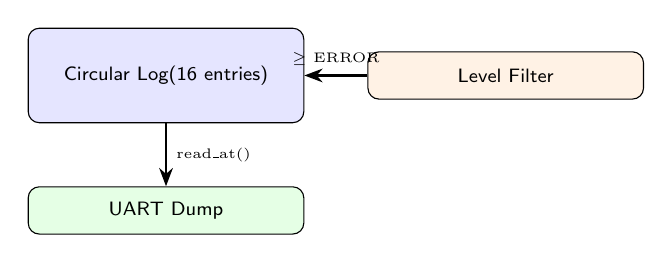
\begin{tikzpicture}[>=Stealth, node distance=0.5cm]
  \node[draw, rounded corners, fill=blue!10,
        minimum width=3.5cm, minimum height=1.2cm,
        font=\scriptsize\sffamily] (log)
    {Circular Log\\(16 entries)};
  \node[draw, rounded corners, fill=green!10,
        minimum width=3.5cm, minimum height=0.6cm,
        font=\scriptsize\sffamily, below=0.8cm of log] (uart)
    {UART Dump};
  \node[draw, rounded corners, fill=orange!10,
        minimum width=3.5cm, minimum height=0.6cm,
        font=\scriptsize\sffamily, right=0.8cm of log] (filt)
    {Level Filter};

  \draw[->, thick] (log) -- node[right, font=\tiny] {read\_at()} (uart);
  \draw[->, thick] (filt) -- node[above, font=\tiny] {$\geq$ ERROR} (log);
\end{tikzpicture}
\end{center}

\vspace{0.5em}
\begin{block}{Log Reading Patterns}
\begin{itemize}
  \item \texttt{read\_latest}: quick check of last event
  \item \texttt{read\_at(0)}: oldest stored entry
  \item \texttt{read\_at(count-1)}: newest entry
  \item Iterate with level filter for error-only dumps
\end{itemize}
\end{block}

\begin{alertblock}{Sequence Gap Detection}
If \texttt{sequence()} returns 100 but \texttt{count()} is 16,
then 84 entries were overwritten. The caller can detect and
report data loss.
\end{alertblock}
\end{column}
\end{columns}
\end{frame}

% ===========================================================================
\section{Embedded Use Case}
% ===========================================================================

\begin{frame}[fragile]{Use Case: FRAM Crash Log with Level Filtering}
\begin{columns}[T]
\begin{column}{0.52\textwidth}
\begin{lstlisting}[style=cstyle,
  title={Persistent crash log in FRAM}]
#include "tiku_kits_ds_circlog.h"

/* Place in FRAM for persistence */
#pragma PERSISTENT(crash_log)
static struct tiku_kits_ds_circlog
    crash_log = {0};

static uint8_t initialized = 0;

void crash_log_init(void)
{
    if (!initialized) {
        tiku_kits_ds_circlog_init(
            &crash_log, 8);
        initialized = 1;
    }
    /* If already initialized, FRAM
       retains previous entries across
       power cycles */
}

void on_watchdog_reset(void)
{
    uint8_t data[] = {0xFF};
    tiku_kits_ds_circlog_append(
        &crash_log,
        TIKU_KITS_DS_CIRCLOG_LEVEL_FATAL,
        TAG_POWER, data, 1);
}

void on_stack_overflow(uint16_t addr)
{
    uint8_t data[2];
    data[0] = (uint8_t)(addr >> 8);
    data[1] = (uint8_t)(addr & 0xFF);
    tiku_kits_ds_circlog_append(
        &crash_log,
        TIKU_KITS_DS_CIRCLOG_LEVEL_FATAL,
        TAG_BOOT, data, 2);
}
\end{lstlisting}
\end{column}

\begin{column}{0.44\textwidth}
\begin{center}
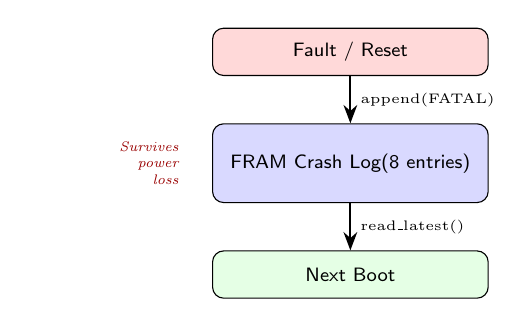
\begin{tikzpicture}[>=Stealth, node distance=0.6cm]
  \node[draw, rounded corners, fill=red!15,
        minimum width=3.5cm, minimum height=0.6cm,
        font=\scriptsize\sffamily] (fault) {Fault / Reset};
  \node[draw, rounded corners, fill=blue!15,
        minimum width=3.5cm, minimum height=1cm,
        font=\scriptsize\sffamily, below=0.6cm of fault] (fram)
    {FRAM Crash Log\\(8 entries)};
  \node[draw, rounded corners, fill=green!10,
        minimum width=3.5cm, minimum height=0.6cm,
        font=\scriptsize\sffamily, below=0.6cm of fram] (boot)
    {Next Boot};

  \draw[->, thick] (fault) -- node[right, font=\tiny] {append(FATAL)} (fram);
  \draw[->, thick] (fram) -- node[right, font=\tiny] {read\_latest()} (boot);

  \node[left=0.3cm of fram, font=\tiny\itshape, text=red!60!black,
        text width=1.8cm, align=right] {Survives\\power\\loss};
\end{tikzpicture}
\end{center}

\vspace{0.5em}
\begin{block}{FRAM Persistence}
\begin{itemize}
  \item \texttt{\#pragma PERSISTENT} places struct in FRAM
  \item Data survives power cycles and resets
  \item On next boot, read entries to diagnose crash
  \item 8 entries = last 8 fatal events
\end{itemize}
\end{block}

\begin{alertblock}{Post-Mortem Analysis}
After a field failure, connect UART and dump the crash log.
Each entry contains a timestamp, fault code, and the
faulting address --- enough to diagnose most issues.
\end{alertblock}
\end{column}
\end{columns}
\end{frame}

% ===========================================================================
\section{Memory Layout}
% ===========================================================================

\begin{frame}{Memory Layout and Entry Sizing}
\begin{columns}[T]
\begin{column}{0.48\textwidth}
\begin{center}
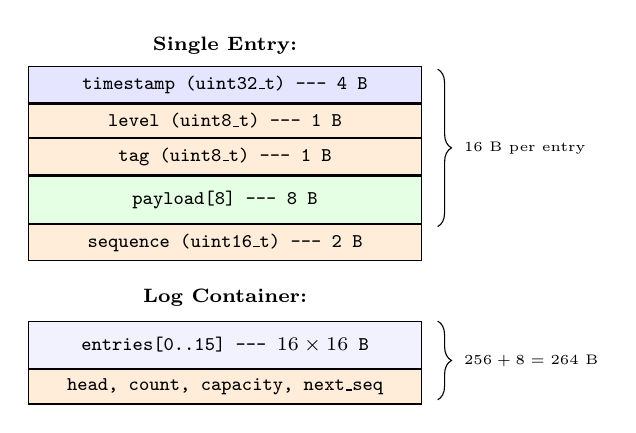
\begin{tikzpicture}[>=Stealth, node distance=0.0cm]
  % Entry structure
  \node[font=\scriptsize\bfseries] at (0, 1.0) {Single Entry:};
  \node[draw, minimum width=5cm, minimum height=0.4cm,
        fill=blue!10, font=\scriptsize\ttfamily] (ts) at (0, 0.5) {timestamp (uint32\_t) --- 4 B};
  \node[draw, minimum width=5cm, minimum height=0.4cm,
        fill=orange!15, font=\scriptsize\ttfamily, below=0cm of ts] (lv) {level (uint8\_t) --- 1 B};
  \node[draw, minimum width=5cm, minimum height=0.4cm,
        fill=orange!15, font=\scriptsize\ttfamily, below=0cm of lv] (tg) {tag (uint8\_t) --- 1 B};
  \node[draw, minimum width=5cm, minimum height=0.6cm,
        fill=green!10, font=\scriptsize\ttfamily, below=0cm of tg] (pl) {payload[8] --- 8 B};
  \node[draw, minimum width=5cm, minimum height=0.4cm,
        fill=orange!15, font=\scriptsize\ttfamily, below=0cm of pl] (sq) {sequence (uint16\_t) --- 2 B};

  \draw[decorate, decoration={brace, amplitude=5pt}]
    (2.7, 0.7) -- (2.7, -1.3)
    node[midway, right=6pt, font=\tiny] {16 B per entry};

  % Log structure
  \node[font=\scriptsize\bfseries] at (0, -2.2) {Log Container:};
  \node[draw, minimum width=5cm, minimum height=0.6cm,
        fill=blue!5, font=\scriptsize\ttfamily] (e0) at (0, -2.8) {entries[0..15] --- $16 \times 16$ B};
  \node[draw, minimum width=5cm, minimum height=0.4cm,
        fill=orange!15, font=\scriptsize\ttfamily, below=0cm of e0] (hd) {head, count, capacity, next\_seq};

  \draw[decorate, decoration={brace, amplitude=5pt}]
    (2.7, -2.5) -- (2.7, -3.5)
    node[midway, right=6pt, font=\tiny] {$256 + 8 = 264$ B};
\end{tikzpicture}
\end{center}
\end{column}

\begin{column}{0.48\textwidth}
\begin{block}{Size Formula}
\[
  \text{Entry} = 4 + 1 + 1 + P + 2 = P + 8 \text{ bytes}
\]
\[
  \text{Total} = C \times (P + 8) + 8 \text{ bytes}
\]
where $C$ = capacity, $P$ = payload size.
\end{block}

\begin{table}
\centering
\scriptsize
\begin{tabular}{@{}rrrr@{}}
\toprule
\textbf{Capacity} & \textbf{Payload} & \textbf{Entry (B)} & \textbf{Total (B)} \\
\midrule
8   & 4  & 12 & 104 \\
8   & 8  & 16 & 136 \\
16  & 8  & 16 & 264 \\
16  & 16 & 24 & 392 \\
32  & 8  & 16 & 520 \\
\bottomrule
\end{tabular}
\end{table}

\vspace{0.3em}
\begin{alertblock}{Payload Size Trade-off}
Larger payloads store more diagnostic data per entry but
consume more FRAM. For crash logs, 4--8 bytes suffices
(fault code + address). For sensor logs, 16 bytes allows
multi-channel data.
\end{alertblock}
\end{column}
\end{columns}
\end{frame}

% ===========================================================================
\section{Complexity}
% ===========================================================================

\begin{frame}{Time and Space Complexity}
\begin{table}
\centering
\begin{tabular}{@{}lcc@{}}
\toprule
\textbf{Operation} & \textbf{Best Case} & \textbf{Worst Case} \\
\midrule
\texttt{init}          & $O(n)$ & $O(n)$ \\
\texttt{append}        & $O(1)$ & $O(1)$ \\
\texttt{read\_latest}  & $O(1)$ & $O(1)$ \\
\texttt{read\_at}      & $O(1)$ & $O(1)$ \\
\texttt{count}         & $O(1)$ & $O(1)$ \\
\texttt{clear}         & $O(n)$ & $O(n)$ \\
\texttt{sequence}      & $O(1)$ & $O(1)$ \\
\bottomrule
\end{tabular}
\end{table}

\vspace{0.5em}
\begin{columns}[T]
\begin{column}{0.48\textwidth}
\begin{block}{Time Analysis}
\begin{itemize}
  \item \texttt{append} writes one entry at the head position,
        copies payload bytes, and increments head via modulo
  \item \texttt{read\_at} computes the physical index from the
        logical index using modulo arithmetic
  \item \texttt{init} and \texttt{clear} are $O(n)$ due to
        \texttt{memset} zeroing the entry array
  \item Iterating all entries: $O(n)$ where $n$ = count
\end{itemize}
\end{block}
\end{column}

\begin{column}{0.48\textwidth}
\begin{block}{Space Analysis}
\begin{itemize}
  \item Fixed: $C \times (P + 8) + 8$ bytes
  \item Independent of total events logged
  \item Bounded: never grows beyond compile-time limit
  \item FRAM-friendly: no fragmentation
  \item Default (16 entries, 8-byte payload): 264 bytes
\end{itemize}
\end{block}
\end{column}
\end{columns}
\end{frame}

% ===========================================================================
\section{Test Suite}
% ===========================================================================

\begin{frame}{Test Cases Overview}
\begin{table}
\centering
\small
\begin{tabular}{@{}clp{7cm}@{}}
\toprule
\textbf{\#} & \textbf{Test Function} & \textbf{What It Verifies} \\
\midrule
1 & \texttt{test\_kits\_ds\_circlog\_init}
  & Initialization, all entries zero, parameter validation \\
2 & \texttt{test\_kits\_ds\_circlog\_append\_read}
  & Append single entry, read\_latest matches, fields correct \\
3 & \texttt{test\_kits\_ds\_circlog\_overwrite}
  & Append beyond capacity overwrites oldest, count stays at cap \\
4 & \texttt{test\_kits\_ds\_circlog\_read\_at}
  & Logical indexing: 0 = oldest, count$-$1 = newest \\
5 & \texttt{test\_kits\_ds\_circlog\_sequence}
  & Sequence monotonically increases, survives overwrite \\
6 & \texttt{test\_kits\_ds\_circlog\_clear}
  & Clear resets count and head, read fails on empty \\
7 & \texttt{test\_kits\_ds\_circlog\_levels\_tags}
  & All log levels stored correctly, tag field preserved \\
8 & \texttt{test\_kits\_ds\_circlog\_payload\_boundary}
  & Payload truncated to PAYLOAD\_SIZE, partial fills zero-padded \\
9 & \texttt{test\_kits\_ds\_circlog\_null\_inputs}
  & All functions reject NULL with ERR\_NULL \\
\bottomrule
\end{tabular}
\end{table}
\end{frame}

% ===========================================================================
\section{Summary}
% ===========================================================================

\begin{frame}{Summary}
\begin{columns}[T]
\begin{column}{0.48\textwidth}
\begin{block}{What We Built}
\begin{itemize}
  \item Circular array of structured log entries
  \item Timestamp, level, tag, payload, sequence per entry
  \item 7 API functions: init, append, read\_latest, read\_at, count, clear, sequence
  \item $O(1)$ append and read operations
  \item Automatic oldest-entry overwrite when full
\end{itemize}
\end{block}

\begin{block}{Key Design Choices}
\begin{itemize}
  \item Silent overwrite --- log never rejects entries
  \item Sequence counter detects missed entries
  \item Configurable payload size and capacity
  \item FRAM-safe static allocation
  \item NULL-pointer validation on all functions
\end{itemize}
\end{block}
\end{column}

\begin{column}{0.48\textwidth}
\begin{block}{Use Cases}
\begin{itemize}
  \item FRAM crash log (survives power loss)
  \item Event tracing with timestamps
  \item Error rate tracking and categorization
  \item Field diagnostic dump via UART
  \item Sensor data journaling
\end{itemize}
\end{block}

\begin{block}{Files}
\scriptsize
\begin{tabular}{@{}lp{4.5cm}@{}}
Common: & \texttt{ds/tiku\_kits\_ds.h} \\
Header: & \texttt{ds/circlog/tiku\_kits\_ds\_circlog.h} \\
Source: & \texttt{ds/circlog/tiku\_kits\_ds\_circlog.c} \\
Tests:  & \texttt{tests/ds/test\_kits\_ds\_circlog.c} \\
\end{tabular}
\end{block}
\end{column}
\end{columns}
\end{frame}

% ---------------------------------------------------------------------------
\begin{frame}{Thank You}
\begin{center}
\Large\textbf{TikuKits DS: Circular Log}\\[0.5em]
\normalsize Structured Event Logging for Physical AI Endpoints\\[1.5em]

\begin{tabular}{rl}
  Repository: & \url{https://github.com/tikuos/tikuOS} \\
  License:    & Apache 2.0 \\
  Common:     & \texttt{tikukits/ds/tiku\_kits\_ds.h} \\
  Header:     & \texttt{tikukits/ds/circlog/tiku\_kits\_ds\_circlog.h} \\
  Source:     & \texttt{tikukits/ds/circlog/tiku\_kits\_ds\_circlog.c} \\
  Tests:      & \texttt{tikukits/tests/ds/test\_kits\_ds\_circlog.c} \\
\end{tabular}
\end{center}
\end{frame}

\end{document}
